\documentclass[11.5pt]{sig-alternate} % sets document style to sig-alternate
% packages
% typesetting
%\usepackage{dirtytalk} % typset quotations easier (\say{stuff})
\usepackage{hanging} % hanging paragraphs
\usepackage[defaultlines=3,all]{nowidow} % avoid widows
\usepackage[pdfpagelabels=false]{hyperref} % produce hypertext links, includes backref and nameref
\usepackage{xurl} % defines url linebreaks, loads url package
\usepackage{microtype}
\usepackage{textgreek}
%\usepackage{textcomp}
%\newcommand{\texttildemid}{\raisebox{0.4ex}{\texttildelow}}
% layout
\usepackage{enumitem} % control layout of itemize, enumerate, description
\usepackage{fancyhdr} % control page headers and footers
\usepackage{float} % improved interface for floating objects
%\usepackage{multicol} % intermix single and multiple column pages
% language
\usepackage[utf8]{inputenc} % accept different input encodings
\usepackage[english]{babel} % multilanguage support
% misc
\usepackage{graphicx} % builds upon graphics package, \includegraphics
%\usepackage{lastpage} % reference number of pages
%\usepackage{comment} % exclude portions of text (?)
\usepackage{xcolor} % color extensions
\usepackage[backend=biber, style=apa]{biblatex} % sophisticated bibliographies % necessary for HTML to display author info and date on abstract page
\usepackage{csquotes} % advanced quotations, makes biblatex happy
\usepackage{authblk} % support for footnote style author/affiliation
% tables and figures
\usepackage{tabularray}
%\usepackage{array} % extend array and tabular environments
\usepackage{caption} % customize captions in figures and tables (rotating captions, sideways captions, etc)
%\usepackage{cuted} % allow mixing of \onecolumn and \twocolumn on same page
\usepackage{multirow} % create tabular cells spanning multiple rows
%\usepackage{subfigure} % deprecated, support for manipulation of small figures
%\usepackage{tabularx} % extension of tabular with column designator "x", creates paragraph-like column whose width automatically expands
%\usepackage{wrapfig} % allows figures or tables to have text wrapped around them
%\usepackage{booktabs} % better rules
% dummy text
%\usepackage{blindtext} % blind text dummy text
%\usepackage{kantlipsum} % Kant style dummy text
\usepackage{lipsum} %lorem ipsum dummy text
% other helpful packages may be booktabs, longtable, longtabu, microtype

\pagestyle{fancy} % sets pagestyle to fancy for fancy headers and footers

% header and footer
% modern way to set header image
\renewcommand{\headrulewidth}{0pt} % defines thickness of line under header
\renewcommand{\footrulewidth}{0pt} % defines thickness of line above header
\setlength\headheight{80.0pt} % sets height between top margin and header image, effectively moves page contents down
\addtolength{\textheight}{-80.0pt} % seems to affect the lower height. maybe only works properly if footer numbers enabled?
\fancyhf{}
\fancyhead[CE, CO]{
\includegraphics[width=\textwidth]{headerImage.png}}
% footer
%\fancyfoot[LE,LO]{Article Title Here \\ DOI: }% left footer article title and doi
%\fancyfoot[CE,CO]{{}} % center footer empty
%\fancyfoot[RE,RO]{\thepage} % right footer page numbers
%\pagenumbering{arabic} % arabic (1, 2, 3) numbering in footer

\hypersetup{colorlinks=true,urlcolor=blue} % sets link color to blue
\urlstyle{same} % sets url typeface to same as rest of text

% set caption and figure to italics, label bold, left align captions, does not transfer to HTML
\captionsetup{labelfont=bf, font={large, it}, justification=raggedright, singlelinecheck=false}
\renewcommand\theContinuedFloat{\alph{ContinuedFloat}}

%this next bit is confusing, but essentially changes the width of the abstract. Seems to have been copied from this https://tex.stackexchange.com/questions/151583/how-to-adjust-the-width-of-abstract
\let\oldabstract\abstract
\let\oldendabstract\endabstract
\makeatletter %changes @ catcode to enable modification (in parsep)
\renewenvironment{abstract} %alters the abstract environment
{\renewenvironment{quotation}%
               {\list{}{\addtolength{\leftmargin}{1em} % change this value to add or remove length to the the default ?
                        \listparindent 1.5em%
                        \itemindent    \listparindent%
                        \rightmargin   \leftmargin%
                        \parsep        \z@ \@plus\p@}%
                \item\relax}%
               {\endlist}%
\oldabstract}
{\oldendabstract}
\makeatother %changes @ catcode to disable modification

% checks
% italics
% links
% dashes
% tildes
\begin{document}
\title{Evidence-based Practices in Mentoring Students with Disabilities: Four Case Studies}

\author[ ]{\large \color{blue} Norma J. Stumbo}
\author[1]{\large \color{blue} Jay K. Martin}
\author[ ]{\large \color{blue} Dan Nordstrom}
\author[ ]{\large \color{blue} Tina Rolfe}
\author[ ]{\large \color{blue} Sheryl Burgstahler}
\author[ ]{\large \color{blue} Jean Whitney}
\author[2]{\large \color{blue} Samantha Langley-Turnbaugh}
\author[ ]{\large \color{blue} Lynn Lovewell}
\author[ ]{\large \color{blue} Babette Moeller}
\author[ ]{\large \color{blue} Randy Larry}
\author[ ]{\large \color{blue} Ed Misquez}


\affil[1]{University of Wisconsin-Madison}
\affil[2]{University of Southern Maine}
\toappear{}

\maketitle
\begin{@twocolumnfalse} 
\begin{abstract}
\item 
\begin{large}
\textit{Individuals with disabilities are attending postsecondary institutions at higher rates than ever before, although many struggle to adjust in college environments. On one hand, higher education positively correlates with better employment outcomes, while on the other, higher education represents more stringent academic requirements and more diffused disability supports. One intervention used to check the ‘trauma’ of transition from high school to postsecondary education is mentoring. This article describes four successful mentorship programs, in various stages of maturity, which are currently funded by the National Science Foundation. The case studies describe the structure of each program, recruitment strategies, the students involved, and outcomes achieved to date. Implications or ‘lessons learned’ are also discussed to provide other important information and impetus for those anticipating such programs.} \\

\end{large} 
\end{abstract}
\end{@twocolumnfalse}

%% ABSTRACT

%% AUTHOR INFORMATION

\textbf{*Corresponding Author, Norma J. Stumbo}\\
\href{mailto:nstumbo@ilinois.edu}{(nstumbo@ilinois.edu)}\\
\textit{Submitted April 14, 2014}\\
\textit{Accepted April 14, 2014}\\
\textit{Published Online April 14, 2014}\\
\textit{DOI: 10.14448/jsesd.03.0003}\\

\pagebreak
\clearpage
\begin{large}
\section*{INTRODUCTION}
Approximately 3 million individuals aged 5 to 15 years old and 24 million individuals aged 16 to 64 years old are experiencing disability in the United States, according the newest American Community Survey (U.S. Bureau of the Census, 2007). Of individuals with disabilities aged 16 to 64, 37.2\% were employed and 30.7\% lived below the poverty line (U.S. Bureau of the Census). These statistics are similar to those reported in 2005, when 38.1 percent of working age adults with disabilities reported working, with only 22.6 percent working full-time for the full year (StatsRRTC, 2005). Jones (1997) and Smith (2007) noted that people with disabilities continue to experience notably lower rates of employment than individuals without disabilities and that targeted interventions are needed to impact these discrepancies.

Mentoring is one example of an intervention that has been promoted for enhancing facilitators and reducing barriers for successful educational and vocational opportunities for people with disabilities (Burgstahler, 2002, 2003, 2006, 2008; Campbell-Whatley, 2001; Campbell-Whatley, Algozzine, \& Obiakor, 1997; Jones, 1997; Kram \& Isabella, 1985; Stumbo, Lindahl-Lewis, \& Blegen, 2008). Mentoring for individuals with disabilities has been widely advocated, although not well-researched or documented (Coombs-Richardson, 2002; Powers, Sowers, \& Stevens, 1995; Snowden, 2003; Stumbo et al.; Sword \& Hill, 2003; Whelley, Radtke, Burgstahler, \& Christ, 2003; Wilson, 2003). DuBois and Rhodes (2006), in establishing a national research agenda for youth mentoring, called for “best practice” program descriptions that produce positive outcomes.

This article describes four related, but independent, mentoring programs for secondary and postsecondary students with disabilities. Descriptions on the overall structure, recruitment strategies, types of students involved, outcomes, and implications are provided for these programs that promote the success of students with disabilities in science, technology, engineering, and mathematics (STEM) education and careers. Each of these four programs provides mentorship experiences as part of a larger suite of programs for students with disabilities. These four projects include the (a) Midwest Alliance in Science, Technology, Engineering, and Mathematics (Midwest) with administrative offices at the University of Wisconsin, the University of Illinois, and the University of Northern Iowa; (b) Northwest Alliance for Acccess to Science, Technology, Engineering, and Mathematics (AccessSTEM) located within the DO-IT Center at the University of Washington; (c) Eastern Alliance for Science, Technology, Engineering, and Math (EAST), located at the University of Southern Maine; and (d) Regional Alliance in Science, Engineering, and Mathematics - Squared: Reaching the Pinnacle (RASEM$^2$/RTP) at New Mexico State University.

\subsection*{Purpose and Benefits of Mentoring Programs for Students with Disabilities}
Mentoring is a relationship between a less experienced individual, called a mentee or protégé, and a more experienced individual known as the mentor (Karcher, Nakkula, \& Harris, 2005; Packard, 2004). Packard (2004) remarked that although the traditional model of mentorships involves a dyadic, face-to-face, long-term connection, it is now widely accepted that mentoring can also be found in various forms, including those at the opposite end of the spectrum—short-term, exclusively electronic, and involving multiple individuals in a ``single" mentorship.

Mentoring relationships, or mentorships, are created in order to provide support and counsel to the mentee or protégé in academic, career, and psychosocial areas (Coombs-Richardson, 2002; Packard, 2004; Rhodes, Grossman, \& Roffman, 2002; Scott \& Homant, 2007-2008) and increase the mentee's ability to navigate through a transition period (Karcher et al., 2005). Typical outcomes of mentorships include improved academic attendance and performance, improved self-worth and self-determination, and access to a close relationship and/or a positive adult role model (Grossman \& Rhodes, 2002; Hamilton \& Hamilton, 2002; Karcher et al.; Loads, Brown, McKenzie, \& Powell, 2006; Rhodes, Grossman, \& Resch, 2000; Rhodes et al., 2002; Rhodes, Reddy, Roffman, \& Grossman, 2005; Rhodes, Spencer, Keller, Liang, \& Noam, 2006). “The idea of mentoring is firmly rooted in the commonsense belief that it is good for a young person to have a close relationship with a caring older person, other than a parent, who can teach and advise and simply be an adult in her or his presence” (Hamilton \& Hamilton, 2002, p. 63).

Mentorships are widely promoted for individuals with disabilities for all the same reasons they are promoted for other individuals, such as learning from positive role models, but they also address additional needs of individuals with disabilities, such as guidance in navigating the lived experience of disability (Coombs-Richardson, 2002; Knight, 2000; Loads et al., 2006; Marsh, 2002; Powers et al., 1995; Snowden, 2003; Sword \& Hill, 2003; Whelley et al., 2003; Wilson, 2003). Mentorships for individuals with disabilities are considered especially important during times of transition such as those from high school to college as well as from post-secondary education to graduate school and professional or vocational employment (Kram \& Isabella, 1985; Powers et al., 2001; Snowden; U.S. Department of Labor, 2006; Weir, 2004; Whelley et al.; Wilson). “The transition from K-12 education to the world of work or higher education is both a trying and exciting time for most young adults, but it can be particularly stressful for students with disabilities” (Wilson, p. 2). Mentorship programs aimed at these periods are designed to ease transitional anxieties, improve social competence, and improve the disability-related skill set and motivation needed to succeed (Burgstahler, 2002, 2003, 2006, 2008; Coombs-Richardson; Powers et al., 1995; Seeger, 2007; Stumbo et al., 2008; Wilson).

It is well known that postsecondary education is a significant pathway for individuals with disabilities to gain better employment, higher income, and a greater quality of life (Bond, Wehman, \& Wittenburg, 2005; Graf \& Whelley, n.d.; Wilson, Getzel, \& Brown, 2000), therefore, mentorship opportunities that enhance students' chances of success in higher education are crucial. This is especially true for science, technology, engineering, and mathematics (STEM) education and careers, in which challenges are even greater for many individuals with disabilities (Burgstahler, 2002, 2003, 2006, 2008; Coombs-Richardson, 2002; Whelley et al., 2003). While students with disabilities share similar concerns about employment, social acceptance, and living independently as students without disabilities, many are often discouraged—both subtly and not so subtly—from studying or entering challenging fields such as those in STEM (Coombs-Richardson). Thus, mentorship programs, designed to address both lifestyle and career issues, are of particular significance and relevance for students with disabilities.

To maximize outcomes, mentorship programs, however, need to be well designed, implemented and evaluated (Grossman \& Rhodes, 2002; Pack\-ard, 2004; Stumbo et al., 2008). An important part of that plan includes details on optimal mentee/mentor selection and matching criteria (Karcher et al., 2005; Viadero, 2006). Consideration needs to be given to mentor and mentee orientation and training concerning their respective roles and expectations as well as the structure of the program (Rhodes et al., 2002). And, importantly, sufficient resources (e.g., time, budget, and staff) need to be allocated to ensure a successful and smooth operation of the experience. Rhodes et al. reported that the most successful programs are those which have adequate supports in place (screening, training, continued oversight, etc.) that enable mentors and mentees to form respectful, high-quality relationships that lead mentees to derive positive benefits from the match.

The lack of these considerations may be one reason why nearly 50 percent of mentorships terminate within the first or second month due to the mentors' feelings of frustration and ineffectiveness (Grossman \& Rhodes, 2002; Karcher et al., 2005). The termination of mentoring relationships often has detrimental effects on the youth who participate (Karcher et al., Rhodes et al., 2005). It is clear, as a number of authors have advocated, that more descriptions of successful mentorship programs need to be detailed in the literature and more and better research needs to be conducted on these efforts (Britner, Balcazar, Blechman, Blinn-Pike, \& Larose, 2006; Karcher et al.; Rhodes, 1994; Rhodes et al., 2002).
 
This article describes and compares four distinct mentorship programs for students with disabilities. Each program is part of a larger set of initiatives designed to help students with disabilities experience success in STEM academic programs and careers. They are associated with regional alliances funded by the National Science Foundation (NSF) for human resource development (HRD) and research in disability education (RDE).

\section*{CASE STUDY \#1:}
\subsection*{The Midwest Alliance in Science, Technology, Engineering, and Mathematics}
\subsubsection*{Structure of the Program}
The Midwest Alliance in STEM offers mentoring opportunities to students and alumni who are current or former residents or students from Wisconsin, Illinois, and Iowa. Using a 16-hour curriculum focusing on building on student strengths and knowledge, the Midwest Alliance pairs students and alumni in one-on-one placements that can be either in-person (also called face-to-face mentoring) or over the internet (also called computer-based mentoring).

Mentees are in high school (grades 9-12) or just starting a postsecondary degree program. Mentors are required to be either enrolled in a postsecondary degree program or a graduate of one. All of the Midwest Alliance's participants must have a verifiable disability as defined by the Americans with Disabilities Act.

Mentors are screened for criminal and sexual based offenses prior to their contact with mentees, using various methods. In Wisconsin and Iowa, the screenings are done through free online services provided by state and local governments. In Illinois, the state police provide a fee-based criminal background check. Sexual based offenses can be checked through the sexual predator registry, which is a nationwide program. The National Mentoring Project is promoting a fee-based background check called Safety-NET, but the program is currently at risk of losing its funding (National Mentoring Project, n. d.).

The Midwest Alliance requires each of its mentors to go through an individualized training session with either an Outreach Coordinator or an assistant. The training program lasts about 45 minutes and can be done in person or over the Internet. Mentors are asked to focus on four major areas during the mentee-mentor relationship: (1) goal setting, (2) self advocacy, (3) requesting accommodations, and (4) study skills.

Once the mentors have been trained, passed their background checks, and have taken the first part of an evaluative survey, one of the project's outreach coordinators places him or her with a mentee.
The placement of mentees and mentors is done with great care, and after significant discussion between staff members and participants. Since the Midwest Alliance is not a tutoring program, it is not necessary that the students have the exact same interests. Rather, outreach coordinators give more weight to the type of accommodations needs that the mentor and mentee share, as well as ensuring that the academic interests of both are in the same general area even though they might not be the same particular discipline. For example, a mentee interested in biomedicine and a mentor majoring in chemistry would still be a good fit according to the Midwest Alliance. A primary consideration in mentee-mentor assignments is the communication strengths of each individual as this determines whether the placement should be computer based, in-person, or perhaps a combination of both.

Each placement is monitored by Midwest Alliance staff periodically throughout the 16 hours of direct time spent between the mentors and mentees. The Midwest Alliance ensures that the participants have a meeting schedule and are making progress, while at the same time allowing for gaps in meeting times due to individual circumstances as they arise. One major incentive for the students to continue their progress is that the first half of their stipend is not disbursed until it is confirmed that their placement is at least half way toward completion.

At the completion of the 16 hours required, participants have the opportunity to reapply or continue their placement. At this juncture, the Midwest Alliance requires that each participant complete a re-test of the survey, which aids in documenting the effects of the mentoring program as well as other aspects of the total student outreach program. Participants are also required to submit a 200- to 300-word description of their experience, which also allows the Midwest Alliance to gain some feedback about the participants' experiences in the mentorship program.

Mentoring participants receive stipends at the completion point of their placements. The amount of the stipend is slightly larger for the mentors than it is for the mentee.

\subsubsection*{Recruitment Strategies}
The Midwest Alliance's recruitment strategy reaches out to numerous stakeholders in nonprofit, professional, educational, and governmental networks and groups. The project utilizes several tactics including direct marketing (email blasts), advertising, event sponsorship and attendance, individual referrals, and publicity. The project's website acts as a vehicle for several of these methods, and it certainly is a major point of entry into student outreach programs. An important recruitment strategy has been the Midwest Alliance's sponsorship of and exhibiting at events (such as assistive technology expos and conferences), as well as through connections with nonprofits that primarily serve youths with disabilities and their parents.

\subsubsection*{Types of Students Involved}
The major types of students that the Midwest Alliance works with in its mentoring program include high school students, post-secondary students, and alumni with disabilities. The youngest participant to date has been 14 years old, and was starting his freshman year in high school. The Midwest Alliance does not currently engage students in 8th grade or younger in its program.

All the participants have a disability of some type. The majority of Midwest Alliance participants have either a specific or nonspecific learning disability, while the second most common type of disability of its participants is either autism or an autism spectrum disorder such as Asperger's syndrome. All other types of disabilities are currently represented among the Midwest Alliance's participants (health disability or illness, mental heath issue or disorder, mobility impairment or physical disability, etc.).

Project participants are from each state in the Midwest Alliance target area (Wisconsin, Illinois, and Iowa). They live in a range of locations, from rural areas and small towns to large metropolitan cities and suburbs, and come from a variety of sociodemographic backgrounds.

\subsubsection*{Impacts/Results/Findings}
The Midwest Alliance has only recently begun to collect quantitative information about the pre-to-post-program changes of its mentorship participants. At the time of this writing, insufficient data has been collected to allow for meaningful synthesis and interpretation. However, the staff have collected qualitative information directly from participants about their mentorship experiences. Although this data has not gained enough “body” to provide definitive evaluative data, individual remarks are illuminating. Below are brief background descriptions and thoughts about the program of three students (pseudonyms are used to protect confidentiality) involved in the Midwest Alliance mentorship program.

\begin{itemize}
    \item Maria was a mentor who, at the time, had recently graduated from the University of Wisconsin-Madison. She was excited and willing to participate in the mentorship program to help others learn about resources and make the college transition easier. To Maria, the most enjoyable and rewarding aspect of the mentorship program included “getting to know the people I worked with.” When asked to describe her mentorship relationship she said it was, “fun in both a professional and friendly way.” Maria took pride in seeing her mentees' confidence levels rise and uncertainty fade related to various aspects of their lives. The biggest challenge she experienced was building a trusting relationship with her mentee and ensuring that it was a “worthwhile relationship.” Maria said the program helped her realize her love of helping others, which is why she began studying for the MCATs with plans to attend medical school.
    \item Timothy, at the time of his first participation in the program, was a freshman at the University of Wisconsin-Whitewater, interested in both physics and engineering. Timothy's first encounter with the Midwest Alliance was through an internship placement in a mechanical engineering lab at the UW-Madison. He spent the summer researching available and needed AT for individuals with physical disabilities and sensory disabilities in STEM educational programs and careers. That fall, while back at UW-Whitewater, Timothy participated as a mentee in the Midwest Alliance program. He said the program made it easier to transition to college, and he learned about accommodations and how to request them. These two experiences were so rewarding that Timothy approached Midwest about helping arrange a second internship placement. Timothy's internship was in a biomedical engineering research lab at UW-Madison, working on a study of bone strength that used computer programs.
    \item Catalina was also a student at the UW-Whitewater. She started out majoring in biology, but switched to psychology. Catalina got involved with the Midwest Alliance as a mentor because of the “huge difference between the way accommodations for people with disabilities are made in high school and the way they are made in college.” When Catalina was a freshman, she was unsure of where to go for help, so she feels that having a mentor during freshman year can be especially helpful. Also, a mentor is someone familiar on campus, someone who has had the same anxieties and knows that it is sometimes not simple to get the accommodations that are needed, especially for those with learning disabilities. Catalina pointed out that “It is nice when your concerns are taken seriously and a mentor is someone that understands those worries.” Catalina valued being a Midwest Alliance mentor and being able to share her experiences, feeling that “it is less lonely living with a disability when you have support from your peers.” She was surprised by the great questions her mentees asked of her. She even wished she had thought to ask some of those questions of her own mentors when she was a mentee! According to Catalina, the Midwest Alliance mentoring program is so helpful that she will definitely participate again, and she encourages others to do so, too.
\end{itemize}

\section*{CASE STUDY \#2}
\subsection*{Northwest Alliance for Acces to Science, Technology, Engineering, and Mathematics}
\subsubsection*{Background and Structure of Program}
Disabilities, Opportunities, Internetworking, and Technology (DO-IT) was founded in 1992 with a grant from the NSF. State funding has allowed DO-IT to institutionalize many of the successful practices funded by NSF as well as by the U.S. Department of Education, the U.S. Department of Labor, and private and corporate sources (DO-IT, n.d.c). DO-IT activities for youth, including the \textit{DO-IT Scholars} and \textit{AccessSTEM} programs, support transitions from high school to college to careers for students with disabilities with interventions that include residential summer programs, on-site and online peer and mentor support, and work-based learning experiences (DO-IT, n.d.a). DO-IT helps participants develop self-determination, social, academic, technology, and career/employment skills. They are guided through critical junctures to degrees and careers. Projects such as \textit{AccessSTEM} are funded by NSF to also increase interest and knowledge in STEM; the model in the Figure provides a timeline for student activities that lead to STEM degrees and careers. Students may enter the program at any stage in the timeline.

This case description focuses on the online, or e-mentoring, community supported by\textit{ AccessSTEM} and other DO-IT programs. Although several electronic tools (e.g., BLOGs, chat) augment communication between participants, email is the primary tool for supporting these connections; through this universally accessible tool, participants of all ability levels can communicate at their own convenience and speed using assistive technology of any type that is often provided by DO-IT. Through the use of Internet discussion lists, mentors and protégés talk about topics of mutual interest. Students learn about STEM college and career fields and about opportunities to gain access to technology and to participate in research and industry internships and other activities. One large list, “doitchat,” includes all community participants, whereas focused groups communicate within smaller groups—e.g., one group focuses on hearing impairments and includes those who are deaf or hard of hearing as well as individuals interested in sign-language, real-time captioning, cochlear implants, and other related issues; another group is for those with an autism spectrum disorder. In another subgroup, “accessstem,” which is sponsored by \textit{AccessSTEM}, students and mentors interested in STEM fields interact. Within all electronic forums, more experienced protégés gradually move into mentoring roles.

A many-to-many style of mentoring is employed in DO-IT's online community. Each participant benefits from the proverbial village of peers, near-peers (where there is an age difference of only a few years), and adult mentors. For example, a high school student who is deaf and interested in studying computer science may hear about the perspectives of several mentors who are computer scientists, from near-peers pursuing college studies in this area, and from fellow high school students interested in the field. If her interests change to biology, different mentors, near-peers, and peers are readily available to her within the community. Support from peers and near-peers provides many of the benefits of encouragement of adult mentors. Being of a similar age and having recently faced many of the same disability-related challenges, near-peers can offer advice and empathy different from that of a traditional adult mentor. In return near-peers gain confidence and leadership skills as they become role models for their peers.

\begin{figure*}[]
    \centering
    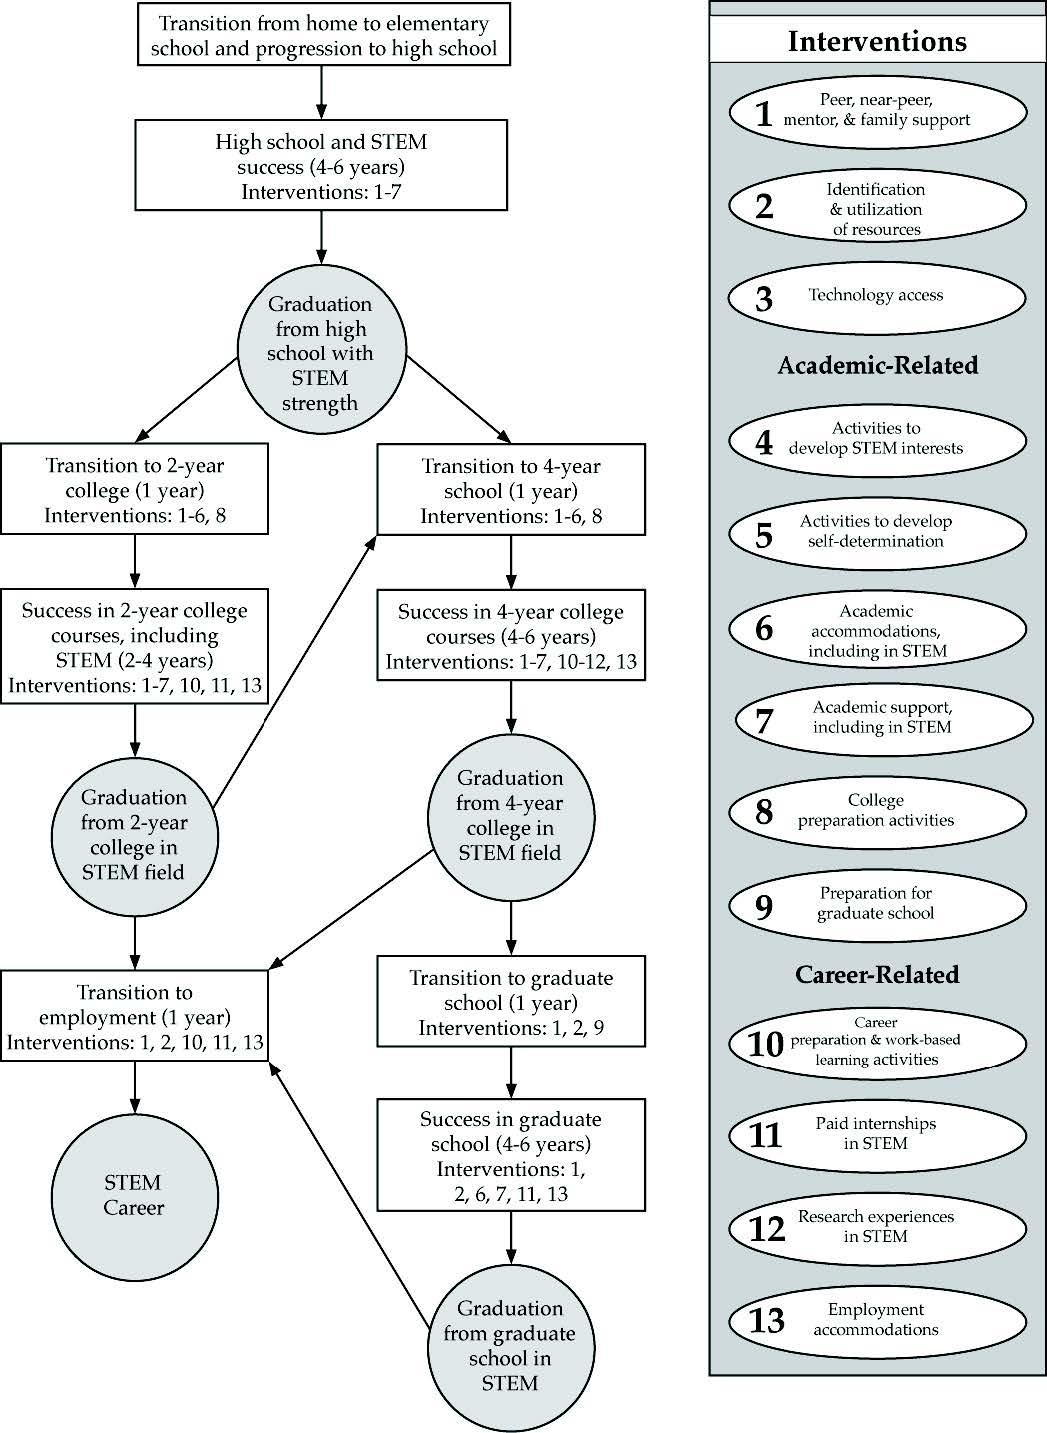
\includegraphics[width=0.9\textwidth]{figure 1.jpg}
    \label{Figure 1}
    \caption{Timeline for Student Activities that Lead to STEM Degrees and Careers}
\end{figure*}

A mentor-protégé and other pairings evolve as participants discover common interests. Project experiences have revealed advantages of the group model over individual mentor-protégé matches to include the following:
\begin{itemize}
    \item Mentor-protégé pairs do not need to be reestablished when the interests of protégés change.
    \item Each student can benefit from perspectives and advice from a large group of mentors.
    \item All participants, not just the one who has a question, benefit from the responses of others.
    \item Mentors can offer specialized input to a large group of protégés without the need to address all transition issues for any single protégé.
    \item Students can gradually learn to offer peer and near-peer support, thereby building confidence and taking on an increasing role as mentors.
    \item Mentors as well as protégés gain perspectives from their participation.
\end{itemize}

Protégés look to the community for advice on assistive technology, school, work, and social situations. As one participant explains, “If I have a problem with any of my special technology, the mentors have been very helpful at getting my technical issues resolved. This is much faster than calling technical support on the phone and sitting on hold while waiting for a technician to answer my call.” This participant, who is blind and uses text-to-speech technology, also appreciates that the advice he receives is in a form he can access using his assistive technology and that he can save messages for later reference.

In this e-mentoring community, members can jump into a discussion or debate at any time. Participants quickly learn that they do not all have the same attitudes or approaches to a problem. Individuals in the community have opportunities to receive and contribute a wide range of opinions and approaches to topics of interest and use self-determination skills to determine a course of action that works best for them. One participant reports, “If I have an issue that I want to get resolved right away, I can write to the mentors and get several responses. This allows me to read each mentor's advice and follow the course of action that I think works best.” In this model the traditional definitions of mentor and protégé are blurred as members both gain from and contribute to the interactions. As one mentor points out, "I am constantly energized by the students I have had the pleasure to communicate with. Their fresh views on issues I struggle with every day help me see that experience can sometimes create unintentional blinders. Fresh views and perspectives are as eye opening to the mentor as to the mentee."

DO-IT's e-community demonstrates the value of long-term relationships as students receive ongoing support for many years and take on increasing levels of mentoring responsibilities for younger participants. For example, while she was in high school, one wheelchair-user met a mentor with a similar level of mobility impairment. The mentor, who is an architect, encouraged the protégé to consider this field. The protégé was admitted into a very competitive school of architecture and ultimately earned a degree.

\subsubsection*{Recruitment Strategies}
Participants are recruited through personal contacts with project participants, parents, partners, and collaborators, online forums, conferences, and newsletters. A key vehicle for promoting this and other student interventions is the \textit{Opportunities!} newsletter, tailored to each postsecondary campus with which the project engages (see samples at \url{http://www.washington.edu/doit/Stem/print.html?ID=335}). This publication, distributed to students with disabilities and advocates, promotes available STEM and college and career preparation offerings at an institution (e.g., STEM lectures, transition fairs); campus disability, technology, tutoring, advising, writing, career planning, and other support services; resources, such as scholarships; and \textit{AccessSTEM} project outreach activities (e.g., mentoring and internships). 

\subsubsection*{Types of Students Involved}
Included in the \textit{AccessSTEM} e-mentoring community are college-bound high school students who face significant challenges in pursuing postsecondary studies and careers as a result of their disabilities. The mentoring community also includes staff and volunteer adult mentors, who are college students and working professionals, most with disabilities themselves.

\subsubsection*{Impacts/Results/Findings}
A rich body of data has been collected on DO-IT interventions for students, including data that reveals the much higher college and career success rates of participants as compared to nation-wide data on other college-capable students with disabilities. The following paragraphs include some of the results related to e-mentoring as reported in an earlier publication (Burgstahler \& Chang, 2007b).

\textit{DO-IT Scholars} have reported that program participation helped them prepare for college and employment; develop Internet, self-advocacy, computer, social, and independent living skills; increase awareness of career options; and increase self-esteem and perseverance (Kim-Rupnow \& Burgstahler, 2004). In post-involvement surveys they reported the greatest effects of the year-round computer and Internet activities to be the development of career skills, followed by academic and social skills. They also reported the development of significant improvements in academic skills, social skills, levels of preparation for college and employment, levels of awareness of career options, and personal characteristics such as perseverance and self-esteem. Further analysis of the data revealed that the perceived career options of female participants increased significantly more than those for male participants (Burgstahler \& Chang, 2007a). In a different survey, parents of \textit{DO-IT Scholars} reported that DO-IT increased their children's interest in college; awareness of career options; self-esteem; and self-advocacy, social, academic, and career/employment skills (Burgstahler, 2002).

DO-IT's experiences demonstrate that the Internet can be used to create and sustain a community that benefits both peers and mentors. An extensive study, funded by the NSF, that included participant surveys and focus groups as well as the content analysis of 12,539 email messages exchanged between 40 \textit{Scholars} and 34 mentors, revealed that participants discussed a wide range of topics that include those related to academics, college transition, careers, computers, assistive technology, STEM, and disability and other personal issues (Burgstahler \& Croheim, 2001). Participants reported that they appreciated the electronic format for its convenience, speed, ability to reach people in remote locations, anonymity, and leveling of social status. They reported positive aspects of using email to include being able to stay close to friends and family; to get answers to specific questions; to meet people from around the world; to communicate quickly, easily, and inexpensively with many people at one time; and to communicate independently without disclosing their disabilities. They predicted that access to the Internet would contribute to their success in college and careers, and reported that peer and mentor relationships furthered their academic and career interests and provided psychosocial, academic, and career benefits. Most protégés reported that DO-IT mentors stimulated their interests in STEM. Reported topics of conversation are wide-ranging— from assistive technology to accommodations to disability legislation and news to personal accomplishments and struggles. In a follow-up e-mentoring study where researchers explored communication differences between males and females, true to gender stereotypes, males were more preoccupied with the Internet and other technology and females with personal issues (Burgstahler \& Doyle, 2005). This result suggests that finding ways to encourage females to develop skills and positive self-concepts in the area of information technology is of critical importance if we are to increase their participation in high tech fields.

Evidence of the efficacy of DO-IT practices is also revealed in its many prestigious awards (DO-IT, n.d.b). Two specifically recognize the value of its e-mentoring community—the President's Award of Excellence for Mentoring in Science, Engineering, and Mathematics fields and the National Information Infrastructure Award for exemplary use of the Internet to further education. Details regarding the creation and management of DO-IT's e-mentoring community are provided in the book, Creating an E- mentoring Community: How DO-IT Does It and How You Can Do It Too (Burgstahler, 2007).

\section*{CASE STUDY \# 3:}
\subsection*{Eastern Alliance for Science, Technology, Engineering, and Mathematics}
\subsubsection*{Structure of Program}
The Eastern Alliance for Science, Technology, Engineering, and Math (EAST) sponsors mentorship of students with disabilities through undergraduate research fellowships (URFs) and online relationships using Mentornet, which is specifically designed to support individuals in science, technology, engineering, and math (STEM) (\url{http://www.mentornet.net/}). This case study describes mentorship through the URFs from the perspective of Sarah (pseudonyms are used to protect confidentiality), a former USM student who was awarded two fellowships and is now pursuing graduate study at University of Massachusetts—Amherst. During the past two summers while earning her BS in Biology at the University of Southern Maine, Sarah, conducted her own research on arachnid (golden orb spider) web weaving under the mentorship of Dr. Christine Maher, associate professor of Biological Sciences Department. Sarah's own research was an incredible feat considering her primary disabilities are health related and include anaphylaxis and asthma, with severe allergies to insect bites/stings, food, and drugs that easily could lead to her death. Nevertheless, her URF provided Sarah the opportunity to test her own limits physically and emotionally: “I really wanted to find out if this was something that I could do, if this was something physically I could do, if this was something that I was up for basically.”

The importance of undergraduate research opportunities in the career development of students in the STEM disciplines has been well documented (Russell, Hancock, \& McCulough, 2007; Wood \& Gentile, 2003; Mervis, 2001). URFs have a positive impact in the areas of student self-confidence and esteem, student motivation to continue the pursuit of STEM academic disciplines and careers, continuation and publication of the research conducted, and the classroom and laboratory instructional practices of the faculty advisors (Langley-Turnbaugh, Locke, Cohen, \& Lightbody, 2007). For many undergraduate students, participation in research represents their first opportunity to transcend what they have learned in formal coursework, and integrate the sometimes seemingly disparate aspects of their academic curricula, providing a capstone experience of considerable value. Undergraduate research experiences can also be paramount in students' decisions to attend graduate school (Gonzalez, 2001; Russell et al.). Finally, because of economic need many Maine students must work during the academic year, in addition to attending classes. As Sarah puts it, “certainly as an undergraduate, you can't just do summer research and not have to pay your bills and not have to do whatever, so I couldn't just spend my life out in a field of spiders without somebody footing the bill.”

EAST's URF program provides stipends to undergraduate students with disabilities majoring in science, technology, engineering, or mathematics, or considering STEM careers, to conduct research with a research supervisor for 8 weeks during the summer. The URF program also provides faculty mentors a stipend for professional development and money for materials and supplies. To receive an URF, students must complete and submit an application, which is usually developed under the guidance of the faculty member who will be the URF mentor. Once an URF is awarded, the student and his or her faculty mentor determine the structure for their work independently and together. The student is the principal investigator and the mentor provides a wide range of support. According to Sarah, “I'm the primary investigator so my responsibilities are pretty much all inclusive, including the experimental design, building of the structure, daily feeding and data collection. Chris has been pretty much instrumental in helping me evaluate the statistical analysis and helping me with the final product.” Sarah described Chris as her “guide,” “sounding board,” and one who provides “emotional support.” Chris is fully aware of Sarah's health concerns. Sarah appreciates the way that Chris shares her vast knowledge of animal behavior, research methodology, and work ethic. Sarah describes Chris as:

\begin{quote}
    “…one of the most hard working people I've known in my entire life. She really, just by her enthusiasm and interest in what she does, she really loves what she does. She has an amazing ethical awareness of what she is doing. She is really good about managing her time and doing the right things by the work. Doing the right things by the project. Not cutting corners when cutting those corners would really kind of cheapen the work or shortcut the work. That is something I really respect. I come from a blue collar family. I come from a hard working family. So people with good work ethic, I get.”
\end{quote}

Other USM faculty have played important collaborative and mentoring roles in Sarah's research in the form of statistical analysis advice, help in growing and anesthetizing “about 10,000 house flies” to feed her spiders, enthusiastic emotional support, and critical advice on research methodology. Of Professor Ken Webber, Sarah said, “you know if you can get a hypothesis past him, it is probably going to be okay. It is probably a good hypothesis.”

Over almost four years of working closely together, Sarah and Chris have evolved into colleagues. They now write together and present at conferences. Sarah credits this relationship to Chris's commitment to the role of mentor that she took on, “she wants to encourage someone to follow into something they love.”

\subsubsection*{Recruitment Strategies}
Since 2003, EAST has awarded a total of 32 Undergraduate Research Fellowships (URFs), which aid in the effort to recruit and sustain undergraduate students with various disabilities in STEM fields. Faculty has been recruited into these research-focused mentoring relationships through presentations at department meetings and at USM's undergraduate research symposium, “Thinking Matters.” At these presentations faculty are introduced to the idea that URFs can be awarded to faculty and student partners to assist faculty with ongoing research projects. Many faculty have had more than one URF and word of mouth has been a major recruitment tool.

Students primarily learn about URFs through presentations in their classes, at workshops, conferences, and through their faculty members. Students are likely to be invited to assist in faculty research or have been working with faculty earning work study funds, prior to applying for an URF. Students are also recruited to apply for URFs when they act as mentors themselves or facilitators at STEM institutes that EAST provides for high school students.

In EAST's program, prospective URF students also need course work that prepares and compliments their participation in hands-on, real-world research. One example of this is a research seminar that provides students direct instruction in defining research problems, experiment design, measurement, sampling, analysis, presentation, and writing for publication (Szymanski, Whitney-Thomas, Marshall, \& Sayger, 1994). Additionally, students also need progressive research experiences so that they can begin their direct participation in undergraduate research under the guidance of a mentor as early in their college career as possible and sustain their participation in URFs as long as possible. To accomplish this, programs might consider structuring two levels of URFs to be awarded at either the assistant or associate level, depending on the students' level of expertise and capacity and the responsibility required by the research project. At the assistant level, students with URFs may participate in a mentor's research, while associate URFs would design and implement their own research under the guidance of their mentor.

\subsubsection*{Types of Students Involved}
In general, students who have participated in EAST are fifty-eight percent (58\%) female, and 42\% male. Ninety-two percent (92\%) of the students are Caucasian. Their primary disability is a learning disability for 42\% of the sample, Attention Deficit Hyperactivity Disorder (ADHD) for 17\% of the sample, a visual impairment or blindness for 17\% of the sample, an orthopedic impairment for 17\% of the sample, and an emotional disability for 8\% of the sample. Eighty-three percent (83\%) of students engaged in EAST activities have participated in at least one research fellowship.

Like many USM students, Sarah came from a background in which college, let alone research and graduate study, were not options that she considered while in high school. She tells us
\begin{quote}
    “I grew up in a poor family where most people went to the military so they didn't end up in worse places. The focus was never on education. I was never told to take the SATs. I never took those. I never took above a business math level math course. I never even took geometry. So college and certainly doctorate programs or even masters programs were something rich people did or other people did.”
\end{quote}
Sarah's high school experience did not set her on a course for postsecondary education and so when she came to USM she began with developmental courses to prepare for college level work. As she tells her story, “It took me three semesters before I could even take a biology class because I couldn't pass the math requirement.”

Nevertheless, Sarah had a natural curiosity about the world around her, which was fostered by her grandmother from a young age. She said, “I think I'd always an amateur naturalist and I just didn't know it. I really do owe a lot to my grandma because she would answer any question you had and if she didn't know the answer, you'd find it out. She was not squeamish in the least and just showed an innate interest and an innate sense of awe and wonder about the world.” When given an opportunity to learn the disciplinary tools to answer her questions about the natural world and provided with the enthusiastic support of a mentor who saw the spark and capacity within Sarah, she flourished and her URF had a powerful effect on her academic and emerging professional life.

\subsubsection*{Impacts/Results/Findings}
Generally speaking, students who participate in EAST activities experience success in postsecondary education and employment in STEM fields. Thirty-three percent (33\%) of the EAST students who graduated from a 4-year college are attending graduate school. Sixty-seven (67\%) of respondents to EAST surveys are currently employed. Thirty-eight percent (38\%) of these held science related positions, another 38\% held technology related positions, and 26\% held positions in education. When asked, EAST students indicated that they found the undergraduate research fellowships very valuable in terms of their preparation for college, graduate schools and/or careers giving the URFs an average rating of 3.70 on a four-point scale (1=not valuable, 4=very valuable) and the mentoring they received an average rating of
3.17 on the same scale.

Sarah is one of the EAST students who graduated from college and is currently pursuing graduate work. As described earlier, Sarah had not considered research, college, and graduate school to be in her future. She credits her URF for the path she is on now saying, “Being able to do my EAST funded research has opened my eyes and my mind to this whole world, I can do something I love. . .that is challenging and fulfilling and I can get paid to do it!”

Sarah's URF and relationship with Chris had a direct impact on her current studies. Through Chris, Sarah has reached out to other researchers in the field. Chris encouraged her to contact other professors, referring Sarah to specific individuals doing related research. Sarah was pleasantly surprised by the reception she received. She described “contacting professors whose work you've read and have them talk to you back and be like ``oh, I'm really excited about your project." That has just been amazing. For me this really has been an incredible life changing experience. It has given me a lot of focus and certainly a lot more forward motion in my life.” Sarah describes the reception that she and her research have received as “validation.” Although her grandmother supported her natural curiosity, Sarah's sense of self-efficacy has grown through this experience and mentorship. She says, “I think this is the first year for me where I've really felt good enough. I think it is because of the interest that people, professors have been like you've got to go on, you've got to do this, this is for you.”

An additional benefit of Sarah's URF has been her growing self-awareness and ability to self-advocate when it comes to her disability-related needs. She describes a summer biology research conference that she attended and the accommodations that she needed to put in place so that she wouldn't be affected by the allergens in the food and the environment. In this situation she was effective in getting a microwave and refrigerator so that she could cook and eat on her own. Her self-advocacy is growing and she is realistic about the challenges that advocacy itself presents. She acknowledges her frustration with how her disability “makes you feel separate from the rest of the group.” She says, however, “Honestly I'm still trying to deal with how to do that [disclose and talk about her needs] and still feel normal because you don't want the only question or conversation at the table to be oh, so you are allergic to what…?”

It is important to note that Sarah also has other disability concerns that go beyond her health needs. Although she is becoming more and more open about her allergies, she is still reluctant to disclose these other disabilities. Nevertheless, Sarah is consciously choosing when, how, to whom, and what she discloses—all of which is evidence of self-determination. Through her undergraduate work, her URFs, and with encouragement from her mentors she has laid a strong foundation upon which to build her growing empowerment.

\section*{CASE STUDY \#4:}
\subsection*{Regional Alliance for Science, Engineering, and Mathematics - Squared/Raising the Pinnacle}
\subsubsection*{Structure of the Program}
The mentorship program was implemented in 1996 and later became the RASEM Squared mentorship program. The project began with the conviction that students with disabilities were more apt to form a relationship with someone closer to their own age than with any staff and faculty. The students (mentees) and mentor both had identified disabilities and the mentors were studying in the science, technology, engineering, and mathematics disciplines.

The first tier is group mentoring. In group mentoring, the Program Coordinator establishes contact and rapport with a teacher or teachers at a particular school. After establishing a good working relationship, the Program Coordinator works with them to incorporate regularly scheduled mentoring activities by RASEM Squared mentors during class time.

Each such instance of mentoring is built around a particular project. The projects incorporate components that vary from in-class instruction to hands-on activities and field trips and often culminate in a final event. At this tier, the mentors themselves are mentored by the teachers, by the Mentor Coordinator, and by each other while they are in turn mentoring the mentees.

The second tier of mentoring involves mentors who have already participated in the tier-one mentoring project. They are ready now to write a mentor project proposal to RASEM Squared/RTP. At this level, the
mentors assume a much greater responsibility for the project and typically schedule project work on a weekend or during regular school hours. Mentees are thus participating in an extracurricular project, run and directed almost entirely by a single RASEM Squared mentor. Parents also have an opportunity to participate and see firsthand how their children are performing.

The value of this two-tiered system is in its step-by-step, hands-on approach to the mentoring process. Successful participation of mentees is ensured and the mentors themselves grow in their professional and personal lives. Also, many more students are reached using this system, since entire classrooms or even schools may participate in the project. The success rate that mentors experience is increased by eliminating the need for the mentees to continually respond electronically to the mentors, and by simplifying the scheduling aspects for all parties involved.

By engaging future engineers and scientists with disabilities as mentors, RASEM Squared/RTP demonstrates a process for encouraging young students with and without disabilities to consider science, technology, engineering, and mathematics fields as careers.

\subsubsection*{Recruitment of Students}
The mentorship program targets local high schools with high minority enrollment as well as other area schools/institutions. High school presentations by RASEM Squared/RTP staff members include oral presentations, videos, and/or mentor project demonstrations.

Field trips for high school students with disabilities to colleges and universities are also used as a recruiting tool. Such activities often include having students as mentors/guides, visiting STEM departments, attending presentations by faculty and staff, and visiting supplemental services at colleges and universities, such as campus services for students with disabilities and financial aid offices. 

Recruitment materials are also mailed to target high schools and postsecondary schools in the RASEM Squared/RTP service area.

Workshops on admissions are available to any students (and their parents) who voice an interest. Information on such workshops is mailed to all area high schools. Activities in the workshops include discussion of career opportunities in STEM fields, mentorship applications, eligibility criteria, and RASEM Squared brochures and other financial aid opportunities.

Mentorship program brochures are also provided to partner institution representatives for high school and college students who have expressed an interest in science, technology, engineering, and mathematics. Partner representatives assist the mentor coordinator with recruitment to stimulate interest in STEM and to solicit potential mentors' participation in educational programs, campus tours, and supplemental programs.

\subsubsection*{Types of Students Involved}
Elementary students work with mentors on various hands-on science and pre-engineering projects. Middle School students work with engineers and contractors who serve as mentors in designing STEM projects. High school students discover the many exciting and rewarding career and educational opportunities available to them in STEM fields. College students have a chance to make industry contacts for obtaining summer jobs, internships, apprenticeships, and full-time employment.

\section*{IMPLICATIONS FOR OTHER PROGRAMS}
The case studies reported in this article suggest a number of implications for the development, implementation, and evaluation of mentorship programs that involve students with disabilities. Implications in six areas will be discussed in greater depth: (a) availability of local role models with disabilities, (b) technology requirements for implementing electronic mentoring programs, (c) need for different delivery styles, (d) value of multiple experiences, (e) need for mentor training, and (e) recognition of investments of time required to build meaningful mentoring relationships and programs.

\subsubsection*{Availability of Local Role Models with Disabilities}
Students with disabilities, especially those with low-incidence disabilities and/or who live in remote areas, have few or no opportunities to meet peers and adults with similar disabilities. These young people benefit from access to supportive relationships that are both face-to-face and over the Internet.

In e-communities they can gain access to a large group of adults and peers with disabilities that are the same or similar to theirs and who are successful in college and professional fields. They soon see that there are people who share some of their experiences and have advice for success in overcoming specific challenges. Through interactions, participants learn about challenges faced by individuals with the same, similar, or different disabilities. In near-peer relationships, students learn from individuals just a year or two ahead of them, in educational progressions and/or in job experiences gives them role models who are successful and make transitions less frightening. Creating an e-mentoring program can enhance outcomes for students with disabilities and provide rewarding experiences for adults with disabilities as well. Mentorships, due to their flexible nature, provide natural and important outlets for interaction, relationship building, and social role development for youth with disabilities.

\subsubsection*{Technology Requirements}
As evidenced by these four case studies, the structure of a mentoring program dictates the type(s) of technology and technological skill needed. E-mail, chat rooms, listservs, and instant messaging all provide rapid connections over great distances . However not all of these technologies are accessible. In cases in which participants do not have access to Internet connections, personal computers, and needed accessible technologies (such as screen readers or voice- recognition software), efforts should be made to provide such access. Specific needs can be determined through direct interviews concerning accommodation needs, project funding, and additional local resources. Training on unfamiliar software and hardware technologies may also be necessary. It is clear that the careful selection of technologies in support of mentoring relationships is a precursor to their success.

\subsubsection*{Need for Varying Delivery Styles}
Another important consideration that emerges from these case studies is that individual needs, styles, and preferences should be considered in structuring the program. For example, some individuals prefer computer-mediated interaction, while others prefer face-to-face communication, while still others prefer some combination of the two. In addition, some individuals prefer one-on-one assignments rather than group discussions.

In addition, in those mentorship programs that have corresponding academic programs, adjunct academic requirements need to be considered as well. For example, students who need to be prepared to participate in research experiences, can work under the guidance of a mentor as early in their academic career as possible and progressively take on higher levels of research activities.

\subsubsection*{Value of Multiple Experiences}
One of the ways to make mentoring more successful is to provide multiple-exposure opportunities for both protégés and mentors. For example, each program discussed in this article describe mentorships that are only one aspect of a larger student outreach program. Activities such as campus tours, community events, summer camps, and internships are provided and mentees and mentors are encouraged to attend and interact. These activities can provide valuable opportunities to network and engage, to learn about resources and opportunities and to experience success. While some of the aforementioned programs offer activities in a specific location, others offer video-conferencing to overcome distance and transportation difficulties. Still other programs offer multiple opportunities for peer-to-peer relationship-building through newsletters, online social networking, undergraduate research conferences, and participation in cohorts of students in common seminars and courses. Once again, the need for flexibility and innovation is clear.

\subsubsection*{Need for Mentor Training}
Training, including orientation materials, for mentors is an important part of mentoring programs. It is important to have clear goals for the protégés and mentors, set expectations and boundaries, share information on communication etiquette and strategies, and to create an environment to cultivate program goals. To maximize the benefits of mentorship relationships, programs should provide mentors with professional development in ways of supporting students with disabilities pursuing STEM studies and careers; the use of technologies as empowerment tools; and the application of the principles of universal design to make STEM education and research more accessible. Orientation can occur in person, over the phone, or online or through a combination of methods. Mentors should be encouraged to introduce themselves and share their interests and experiences, be open minded, encourage participants to share their perspectives, and to help protégés develop self-determination skills. In addition, protégés should learn about Internet and in-person safety, and steps they can take to protect themselves.

\subsubsection*{Investments in Time}
It should be emphasized that being flexible, innovative, and needs-based in the development of a mentoring program requires a considerable investment in time from the program staff as well as the participants. Staff should allow the needs of the participants to direct a number of program design decisions, such as selecting modes of delivery (e-mentoring, face-to-face mentoring, complementary activities for multiple exposures), and technologies. Staff time is needed to develop ``menus" of program options before protégés and mentors are recruited, for training mentors and mentees, and for trouble-shooting and problem-solving as mentoring relationships unfold. Considerable staff time is needed for launching, monitoring, and maintaining the pro- gram. Both quantitative and qualitative data should be collected as part of the program evaluation. Both mentees and mentors also need to invest a meaningful amount of time to make the mentoring relationship worthwhile and productive. Setting clear goals, expectations, and boundaries is helpful to both mentees and mentors for staying on track and keeping the mentorship focused.

\section*{SUMMARY}
This article describes four mentorship programs varying in structure and location, but sharing a common goal of helping students with disabilities make successful transitions to postsecondary education and careers. These programs, in various stages of maturity, offer insights to others who are contemplating the initiation of mentoring programs for individuals with disabilities. Six implication areas that emerge from these case studies are: (a) availability of local role models with disabilities, (b) technology requirements for implementing electronic mentoring programs, (c) need for different delivery styles, (d) value of multiple exposures, (e) need for mentor training, and (f) recognition of investments of time required to build meaningful mentoring relationships and programs. Conceivably, these promising practices can help launch other firmly grounded, successfully functioning mentoring programs.

\textbf{Disclaimer:} The information contained in this publication is based upon work supported by the National Science Foundation under Grant No. HRD-0533197, and Cooperative Agreements \#HRD-0227995, \#HRD-0833338, \#HRD-0833567, and \#HRD-0622930. Any opinions, findings, and conclusions or recommendations expressed in this material are those of the author(s) and do not necessarily reflect the views of the National Science Foundation.

\section*{AUTHOR INFO}
\textbf{Norma J. Stumbo}\\
Research Director, Midwest Alliance in Science, Technology, Engineering, and Mathematics (Midwest Alliance)\\
University of Illinois\\
\href{mailto:nstumbo@illinois.edu}{nstumbo@illinois.edu}\\

\textbf{Jay K. Martin}\\
Professor, Mechanical Engineering\\
Principal Investigator, Midwest Alliance\\
Director, UW-CREATe (Center for Rehabilitation Engineering and Assistive Technology)\\
University of Wisconsin-Madison\\

\textbf{Dan Nordstrom}\\
Midwest Alliance in Science, Technology, Engineering, and Mathematics (Midwest)\\

\textbf{Tina Rolfe}\\
Midwest Alliance in Science, Technology, Engineering, and Mathematics (Midwest)\\

\textbf{Sheryl Burgstahler}\\
Northwest Alliance for Access to Science, Technology, Engineering, and Mathematics (Access\-STEM)\\

\textbf{Jean Whitney}\\
Eastern Alliance for Science, Technology, Engineering, and Mathematics (EAST)\\

\textbf{Samantha Langley-Turnbaugh}\\
Eastern Alliance for Science, Technology, Engineering, and Mathematics (EAST)\\

\textbf{Lynn Lovewell}\\
Eastern Alliance for Science, Technology, Engineering, and Mathematics (EAST)\\

\textbf{Babette Moeller}\\
Eastern Alliance for Science, Technology, Engineering, and Mathematics (EAST)\\

\textbf{Randy Larry}\\
Regional Alliance for Science, Engineering, and Mathematics - Squared: Reaching the Pinnacle (RASEM2/RTP)\\

\end{large}
\clearpage
\section*{REFERENCES}\par 

\leftskip 0.25in
\parindent -0.25in 
%%%
Bond, G. R., Wehman, P., \& Wittenburg, D. (2005). \textit{Evidence-based practices that promote employment of people with disabilities}. Unpublished paper. Washington, D.C.: National Council on Disability.

Britner, P. A., Balcazar, F. E., Blechman, E. A., Blinn-Pike, L., \& Larose, S. (2006). Mentoring special youth populations. \textit{Journal of Community Psychology, 34}(6), 747-763.

Burgstahler, S. (2002). The value of DO-IT to kids who did it!\textit{ Exceptional Parent, 32}(11), 79-86.

Burgstahler, S. (2003). DO-IT: Helping students with disabilities transition to college and careers. \textit{Research Into Practice Brief, 2}(3), 6 pages (on- line).

Burgstahler, S. (2006, August). Creating an e-mentoring community. \textit{Information Brief, 5}(4), 1-
5.

Burgstahler, S. (2007).\textit{ Creating an e-mentoring community: How DO-IT does it and how you can do it too. Seattle: University of Washington}. Retrieved October 10, 2008, from \url{http://www.washington.edu/doit/Mentor}

Burgstahler, S. (2008).\textit{ Opening doors: Mentoring on the Internet. Seattle: University of Washington}. Retrieved October 10, 2008, from \url{http://www.washington.edu/doit/Brochures/Techn ology/doors.html}

Burgstahler, S., \& Chang, C. (2007a). Gender differences in perceived value of components of a program to promote academic and career success for students with disabilities. \textit{Journal of Science Education for Students with Disabilities, 12}(1), 1- 11.

Burgstahler, S., \& Chang, C. (2007b). \textit{A preliminary report of the AccessSTEM/DO-IT longitudinal transition study (ALTS)}. Retrieved October 10, 2008, from \url{http://www.washington.edu/doit/Stem/}

Burgstahler, S., \& Croheim, D. (2001). Supporting peer-peer and mentor-protégé relationships on the Internet. \textit{Journal of Research on Technology in Education, 34}(1), 58-74.

Burgstahler, S., \& Doyle, A. (2005). Gender differences in computer-mediated communication among adolescents with disabilities: Science, technology, engineering, and mathematics case study. \textit{Disability Studies Quarterly, 25}(2). Retrieved October 10, 2008, from \url{http://www.dsq- sds.org/2005_spring_toc.html}

Campbell-Whatley, G. D. (2001). Mentoring students with mild disabilities: The “nuts and bolts” of program development. \textit{Intervention in School and Clinic, 36}(4), 211-216.

Campbell-Whatley, G. D., Algozzine, B., \& Obiakor, F. (1997). Using mentoring to improve academic programming for African American male youths with mild disabilities. \textit{School Counselor, 44}(5), 362-367.

Coombs-Richardson, R. (2002). Mentoring and constructivism: Preparing students with disabilities for careers in science.\textit{ Proceedings of the Annual International Conference of the Association for the Education of Teachers in Science (Charlotte, NC, January 10-13, 2002)}.

Disabilities, Opportunities, Internetworking, and Technology (DO-IT). (n.d.a).\textit{ DO-IT awards}. Seattle: University of Washington. Retrieved October 10, 2008, from \url{http://www.washington.edu/doit/Award/}

DO-IT. (n.d.b) \textit{DO-IT programs and projects}. Seattle: University of Washington. Retrieved October 10, 2008, from \url{http://www.washington.edu/doit/Programs/}

DO-IT. (n.d.c).\textit{ DO-IT support}. Seattle: University of Washington. Retrieved October 10, 2008, from \url{http://www.washington.edu/doit/Support/}

DuBois, D. L., \& Rhodes, J. E. (2006). Introduction to the special issue: Youth mentoring: Bridging science with practice. \textit{Journal of Community Psychology, 34}(6), 647-655.

González, C., (2001, August 31). Undergraduate research, graduate mentoring, and the university's mission. \textit{Trends in Undergraduate Education}. Retrieved March 11, 2008, from \url{www.sciencemag.org}

Graf, J., \& Whelley, T. (n.d.). \textit{Success for people with disabilities after postsecondary education.} Available online from \url{www.rrtc.hawaii.edu/products/phases/phase2/stud y17.html}

Grossman, J. B. \& Rhodes, J. E. (2002). The test of time: Predictors and effects of duration in youth mentoring relationships.\textit{ American Journal of Community Psychology, 30}(2), 199-219.

Grossman, J. B., Roffman, J., \& Rhodes, J. E. (2002). The rhetoric and reality of youth mentoring. \textit{New Directions for Youth Development, 93}, 9-20.

Hamilton, M. A., \& Hamilton, S. F. (2002). Why mentoring in the workplace works. \textit{New Directions for Youth Development, 93}, 59-89.

Jones, G. E. (1997). Advancement opportunity issues for persons with disabilities. \textit{Human Resource Management Review, 7}(1), 55-76.

Karcher, M. J., Nakkula, M. J., \& Harris, J. (2005). Developmental mentoring match characteristics: Correspondence between mentors' and mentees' assessments of relationship quality. \textit{The Journal of Primary Prevention, 26}(2), 93-110.

Kim-Rupnow, W. S., \& Burgstahler, S. (2004). Perceptions of students with disabilities regarding the value of technology-based support activities on postsecondary education and employment. \textit{Journal of Special Education Technology, 19}(2). Retrieved October 10, 2008 from \url{http://jset.unlv.edu/19.2/rupnow/first.html}

Knight, T. M. (2000). Planting the seeds of success: Advising college students with disabilities. \textit{The Mentor: An Academic Advising Journal, 2}(2), 4 pages (on-line).

Kram, K. E., \& Isabella, L. A. (1985). Mentoring alternatives: The role of peer relationships in career development.\textit{ Academy of Management Journal, 28}(1), 110-132.

Langley-Turnbaugh, S.J., Locke, S., Cohen, L., \& Lightbody, N. (2007). Research experiences for undergraduates with disabilities in science, technology, engineering, and mathematics (STEM) majors. In K. K. Karakstis and T. Elgren (Eds). \textit{How to design, implement, and sustain a research-supportive undergraduate curriculum} (pp. 45-56). Washington, D.C.: NSF Council for Undergraduate Research.

Loads, D., Brown, M., McKenzie, K., \& Powell, H. (2006). Developing mentorship through collaboration. \textit{Learning Disability Practice, 9}(3), 16-18.

Marsh, M. M. (2002). The influence of discourses on the precarious nature of mentoring. \textit{Reflective Practice, 3}(1), 103-115.

Mervis, J. (2001, August 31). Student research: What is it good for?\textit{ Science, 293}(5535), 1614- 1615.

National Mentoring Project. (n.d.).\textit{ MENTOR’s SafetyNET program: Safety net extension}. Retrieved August 19, 2008 from \url{http://apps.mentoring.org/safetynet/}

Packard, B. W. (2004).\textit{ Definition of mentoring}. Retrieved September 16, 2008, from: \url{http://ehrweb.aaas.org/sciMEntoring/Mentor_Defi nitions_Packard.pdf}

Padron, J. M. (2006). Experience with post-secondary education for individuals with severe mental illness. \textit{Psychiatric Rehabilitation Journal, 30}, 147-149.

Powers, L. E., Sowers, J., \& Stevens, T. (1995). An exploratory, randomized study of the impact of mentoring on the self-efficacy and community- based knowledge of adolescents with severe physical challenges. \textit{Journal of Rehabilitation, 61}(1), 33-41.

Powers, L. E. Turner, A., Ellison, R., Matuszewski, J., Wilson, R., Phillips, A., et al. (2001). A multi-component intervention to promote adolescent self-determination. \textit{Journal of Rehabilitation, 67}(4), 13-19.

Rhodes, J. E. (1994). Older and wiser: Mentoring relationships in childhood and adolescence. \textit{Journal of Primary Prevention, 14}(3), 187-196.

Rhodes, J. E., Grossman, J. B., \& Resch, N. L. (2000). Agents of change: Pathways through which mentoring relationships influence adolescents' academic adjustment. \textit{Child Development, 71}(6), 1662-1671.

Rhodes, J. E., Grossman, J. B., \& Roffman, J. (2002). The rhetoric and reality of youth mentoring. \textit{New Directions for Youth Development, 93}, 9- 20.

Rhodes, J., Reddy, R., Roffman, J., \& Grossman, J. B. (2005). Promoting successful youth mentoring relationships: A preliminary screening questionnaire. \textit{The Journal of Primary Prevention, 26}(2), 147-167.

Rhodes, J. E., Spencer, R., Keller, T. E., Liang, B., \& Noam, G. (2006). A model for the influence of mentoring relationship on youth development. \textit{Journal of Community Psychology, 34}(6), 691-707.

Russell, S., Hancock, M., McCullough, J., (2007, April 27). Benefits of undergraduate research experiences. \textit{Education Forum}. Retrieved March 11, 2008 from \url{www.sciencemag.org.}

Scott, C. L., \& Homant, R. J. (2007-2008). The professional mentor program plus: An academic success and retention tool for adult learners. \textit{Journal of College Student Retention: Research, Theory, and Practice, 91}(1), 61-73.

Seeger, K. L. (2007). \textit{Mentoring youth with disabilities: The mentor’s lived experience}. Thesis, Louisiana State University and Agricultural and Mechanical College.

Smith, D. L. (2007). The relationship of type of disability and employment status in the United States from the behavioral risk factors surveillance system. \textit{Journal of Rehabilitation, 73}(2), 32-40.

Snowden, R. (2003). Partners for youth with disabilities. \textit{American Rehabilitation, 27}(1), 36-41.

StatsRRTC. (2005). \textit{2005 Disability Status Reports United States}. Ithaca, NY: Cornell University.

Stumbo, N.J., Lindahl-Lewis, P., \& Blegen, A. R. (2008). Two mentorship case studies of high school and university students with disabilities: Milestones and lessons. \textit{Journal of Rehabilitation, 74}(3), 45-51.

Sword, C., \& Hill, K. (2003). Creating mentoring opportunities for youth with disabilities: Issues and suggested strategies.\textit{ American Rehabilitation, 27}(1), 14-17.

Szymanski, E., Whitney-Thomas, J., Marshall, L., \& Sayger, T. (1994). The effect of graduate instruction in research methodology on research self-efficacy and perceived research utility. \textit{Rehabilitation Education, 8}, 319-331.

U.S. Bureau of the Census. (2007).\textit{ American community survey summary tables}. Retrieved October 20, 2008 from \url{www.census.gov/hhes/www/disability/data_title.html}

U.S. Department of Labor. (2006). \textit{Cultivating leadership: Mentoring youth with disabilities}. Retrieved October 21, 2008 from \url{www.dol.gov/odep/pubs/fact/cultivate.html}

Viadero, D. (2006). Rise of youth mentoring out- paces knowledge base.\textit{ Education Week, 26}(15), 8-9.

Weir, C. (2004). Person-centered and collaborative supports for college success. \textit{Education and Training in Developmental Disabilities, 39}(1), 67-73.

Whelley, T. A., Radtke, R., Burgstahler, S., \& Christ, T. W. (2003). Mentors, advisers, role models and peer supporters: Career development relationships with individuals with disabilities. \textit{American Rehabilitation, 27}(1), 42-49.

Wilson, J. (2003). Mentors: Paving the transition from school to adulthood for students with disabilities. \textit{American Rehabilitation, 27}(1), 2,52.

Wilson, K., Getzel, E., \& Brown, T. (2000). Enhancing the post-secondary campus climate for students with disabilities.\textit{ Journal of Vocational Rehabilitation, 14}, 37-50.

Wood, W. B. \& Gentile, J. M. (2003, November 28). Teaching in a research context.\textit{ Science, 302}(5650), 1510.

\end{document}
